% !TEX root = ../main_orange.tex

The ATLAS open data consist in a set of MC and real events that the ATLAS collaboration has released for open use. The main web page where they are introduced is \url{http://atlas.cern/resources/opendata}. Please spend some time on this page, explore it, play with it.

The next step is to actually do something. In the ``Online Open Data Analysis'' section of the page, click on ``Analyse ATLAS Open Data with Jupyter Notebooks''. You should get to this \href{https://mybinder.org/v2/gh/atlas-outreach-data-tools/notebooks-collection-opendata/master/}{page}. Now select \verb|13-TeV-examples|, then \verb|uproot_python|. Each notebook corresponds to a different analysis. Please open \verb|HZZAnalysis.ipynb|, and read it through. The notebook should work (if it does not, please get in touch with one of the tutors). 

Let's dissect what this notebook does. 

\section{Review of the jupyter notebook step by step}
\label{sec:review_notebook}

\begin{itemize}
\item The first cell is a technical one, and it takes care of installing a number of modules that may not be available on the machine. In particular note the module \verb|uproot|, which is the one that will allow us to decouple completely from \href{https://root.cern.ch/}{root}, despite the open data being physically saved as \verb|root| files. 

\item The second cell imports a number of modules which will be necessary for the analysis. You should be more or less familiar with everything, with the possible exception of \verb|uproot|. Google is your friend, please have a look at any module you are not specifically familiar with. 

\item The third cell contains a few important things. First of all, it specifies two float numbers (\verb|lumi| and \verb|fraction|). \verb|lumi| specifies what total \Lint the data that we will be using correspond to ($10\ \ifb$ in this case). Running on all data can take time. In case you only want to quickly check whether your code is working, you can only run on a \verb|fraction| of all available data. 

Finally (very important!), \verb|tuple_path| specifies where the data and simulated samples are. This example uses the input samples from a web location. Depending on the quality of your connection and the storage capabilities of your machine, you may find faster to download the samples to your machine and run locally on them. 

The location specified is actually browsable. You can copy \url{https://atlas-opendata.web.cern.ch/atlas-opendata/samples/2020/4lep/} in a new browser tab. As the link suggests, this folder contains events containing four leptons. There are two subfolders, \verb|Data| and \verb|MC|. I am sure you guessed already what they contain. Let's explore the \verb|Data| one first. This is not very interesting: the available data are split in four files. A lot more interesting is the \verb|MC| one. It contains simulated collisions yielding specific processes. A word on the naming convention: 

\begin{itemize} 
\item \verb|mc| at the beginning specifies these are MC samples. 
\item the number that follows is a unique numerical identifier of the sample, called \textit{dataset identifier}, or DSID. 
\item then you have a string that characterises the process. For example, \verb|WH125_ZZ4lep| means this is a process where $WH$ is produced, the Higgs boson decays into two $Z$ bosons, which in turn produce four leptons. 
\item \verb|4lep| means.... well, you know. 
\item the \verb|root| extension specifies the type of file. 
\end{itemize}  

In related folders, you also have other types of events. If you go to \url{https://atlas-opendata.web.cern.ch/atlas-opendata/samples/2020/} you will get an overview of what type of events are available. We will be using those with two and three leptons in our bonus exercise. 

\item The fourth cell defines a dictionary for the samples we will be using, exploiting one of the field of the MC naming convention discussed above. This analysis will look for $pp\rightarrow H\rightarrow ZZ\rightarrow 4\ell$. In this context, ``signal'' is any process that contains a Higgs boson production giving four leptons in the final state. The ``background'' is any other SM process that would yield four leptons in the final state. The main contribution to the background is the production of two $Z$ bosons, and that is why this process is singled out. Other processes that could give four leptons are listed separately.

\begin{remark}
You may wonder how, for example, \verb|Zee| (that is $Z$ boson production followed by $Z\rightarrow e^+e^-$) can give four leptons in the final state. That is a very good question, and it gives the chance to introduce the concept of \textit{reducible} and \textit{irreducible} background. $pp\rightarrow ZZ \rightarrow 4 \ell$ is an irreducible background to our Higgs analysis, because it gives a final state with the same particle content of our signal. $Z\rightarrow e^+e^-$ is a reducible background. That means it normally does not produce a final state with the same particle content as the signal, but because of rare features (either physical, or from the detector), it may actually yield the same final state. In this case, in a small fraction of events one of the electrons in the final state may radiate a photon that could convert in a second electron pair. 
\end{remark}

\item The fifth cell creates a function to loop over the data and MC samples, relying on a \verb|read_file()| function that will be defined later. 
\item The next two cells define the \verb|calc_weight| and \verb|get_xsec_weight| functions. The MC events need a series of corrections to truthfully represent the data. For example, the electron identification efficiency predicted by the plain MC might be a bit optimistic or pessimistic with respect to that that we have with the real detector. Therefore the MC is corrected with a factor \verb|scaleFactor_ELE| to take this into account. The other factors appearing in the \verb|calc_weight| have similar explanations. \verb|xsec_weight| deserves a dedicated explanation 

\begin{definition}
\textbf{Cross-section weight:} Suppose that I simulate $N$ events of a process whose cross-section is $\sigma$. I know that the data I will be looking at correspond to an integrated luminosity $L$. To help understanding, let's use some numbers: $\sigma = 10$ fb, $L = 10\ \ifb$, $N = 100000$. I now want to use my $N$ MC events to predict the yields in data. Clearly I need to rescale my MC events in some way. I will need to apply a multiplicative weight $w$ to each of my $N$ events such that they will eventually represent the number of events I expect in data, that is (see Section~\ref{sec:cross_section_lumi}) $N_{\mathrm{data}} = \sigma \times L$

\begin{align*} 
wN &= N_{\mathrm{data}} = \sigma \times L \\ 
w &= \frac{\sigma \times L}{N}
\end{align*} 

With our specific numbers above: we expect $N_{\mathrm{data}} = 100$ events in data, and we have $N = 100000$ to represent them. We should therefore multiply our $N$ MC events by $w = N_{\mathrm{data}}/N = 10^{-3}$. 
\end{definition}

That is in essence what is in these cells, with just slight differences. 

\item The next cell simply defines to compute the invariant mass of the leading four leptons in the event. 

\begin{exercise}
From the definition of invariant mass in Section~\ref{sec:invariant_mass} and the definition of $\eta, \phi, \pt$ in Section~\ref{sec:collider_physics_variables}, show that the calculation in this cell is correct. 
\end{exercise}


\item The next cell defines two boolean functions (that is, functions whose outcome is either True or False) that will later be used to filter the events. 
\item The next cell does most of the work using the function defined earlier. This defines the function \verb|read_file()| mentioned in the sixth cell. The inline comments present there should help understanding what is going on. In case you still have questions, please get in touch with one of the tutors. 
\item The last cell shows a possible way of plotting the results. 
\end{itemize}

The jupyter notebook examples just discussed can be found in the git repository at \href{https://github.com/atlas-outreach-data-tools/notebooks-collection-opendata}{this link} (it can also be reached by clicking on the top-right corner button \verb|Visit Repo|). You should be able to download and execute them. A number of other examples (in the form of python modules and scripts) can be found at \href{https://github.com/atlas-outreach-data-tools/atlas-outreach-Python-uproot-framework-13tev}{this other git repository}. This portfolio of examples should give a wide range of answers to possible questions that you might have when trying to do the experiments proposed in Section~\ref{sec:experiments}. 

By the way, it is worth to spend the time to digest the result of the analysis outlined above: the plot (repeated here in Figure~\ref{fig:H_4lep}) shows the invariant mass of the four leptons in events with four leptons. The red and purple histograms represent the prediction from the MC for the irreducible and reducible backgrounds, respectively. One notices a peak at 90 GeV, nicely predicted by the $ZZ$ MC: 90 GeV is the mass of the $Z$ boson. These events correspond to cases where the four leptons all come from one $Z$ boson. A second feature of the $ZZ$ prediction is a step at about 180 GeV. That is the mass of two $Z$ bosons: most events where the $Z$ bosons are emitted on shell are forced to yield an invariant mass above two times the $Z$ boson mass. The irreducible background is \textit{non-resonant}, that is, does not have a peak at any specific value of the invariant mass.

A small peak at 125 GeV in the data can be observed. Congratulations: you have just re-discovered the Higgs boson in its decay into four leptons! 

\begin{figure}[tb] 
	\centering
	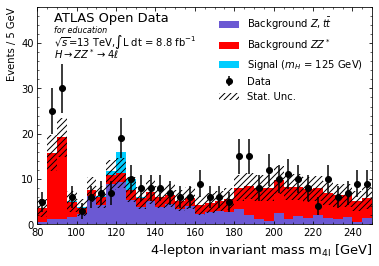
\includegraphics[width=0.5\columnwidth]{Figures/H_4lep.png}
	\label{fig:H_4lep}
	\caption{Result of the example analysis described in the text. A Higgs boson peak in the four-lepton invariant mass is visible at $ m \sim 125\ \GeV$.}
\end{figure}

\section{ATLAS Open Data: Getting Started} 


Although the jupyter notebook example is a good starting point to understand the mechanics of what we are going to do, we will need to have more freedom in what we do. Anaconda is a great framework to do this. You can start by cloning the git repository at \href{https://github.com/atlas-outreach-data-tools/atlas-outreach-Python-uproot-framework-13tev}{this link}. From the terminal window, or Anaconda prompts type

\begin{verbatim}
git clone https://github.com/atlas-outreach-data-tools/atlas-outreach-Python-uproot-framework-13tev
\end{verbatim}

You can now execute HZZAnalysis.py. For example

\begin{verbatim}
python3  HZZAnalysis.py
\end{verbatim}

Now be patient. The running may take few minutes. If everything is smooth, you should see something like Figure~\ref{fig:running_HZZ}. Of course the numbers corresponding to the time taken to run on a given sample may change depending on your machine and connection. For example: on my machine it took few seconds to run on data, but some minutes to run on \verb|llll|. 

\begin{figure}[tb] 
	\centering
	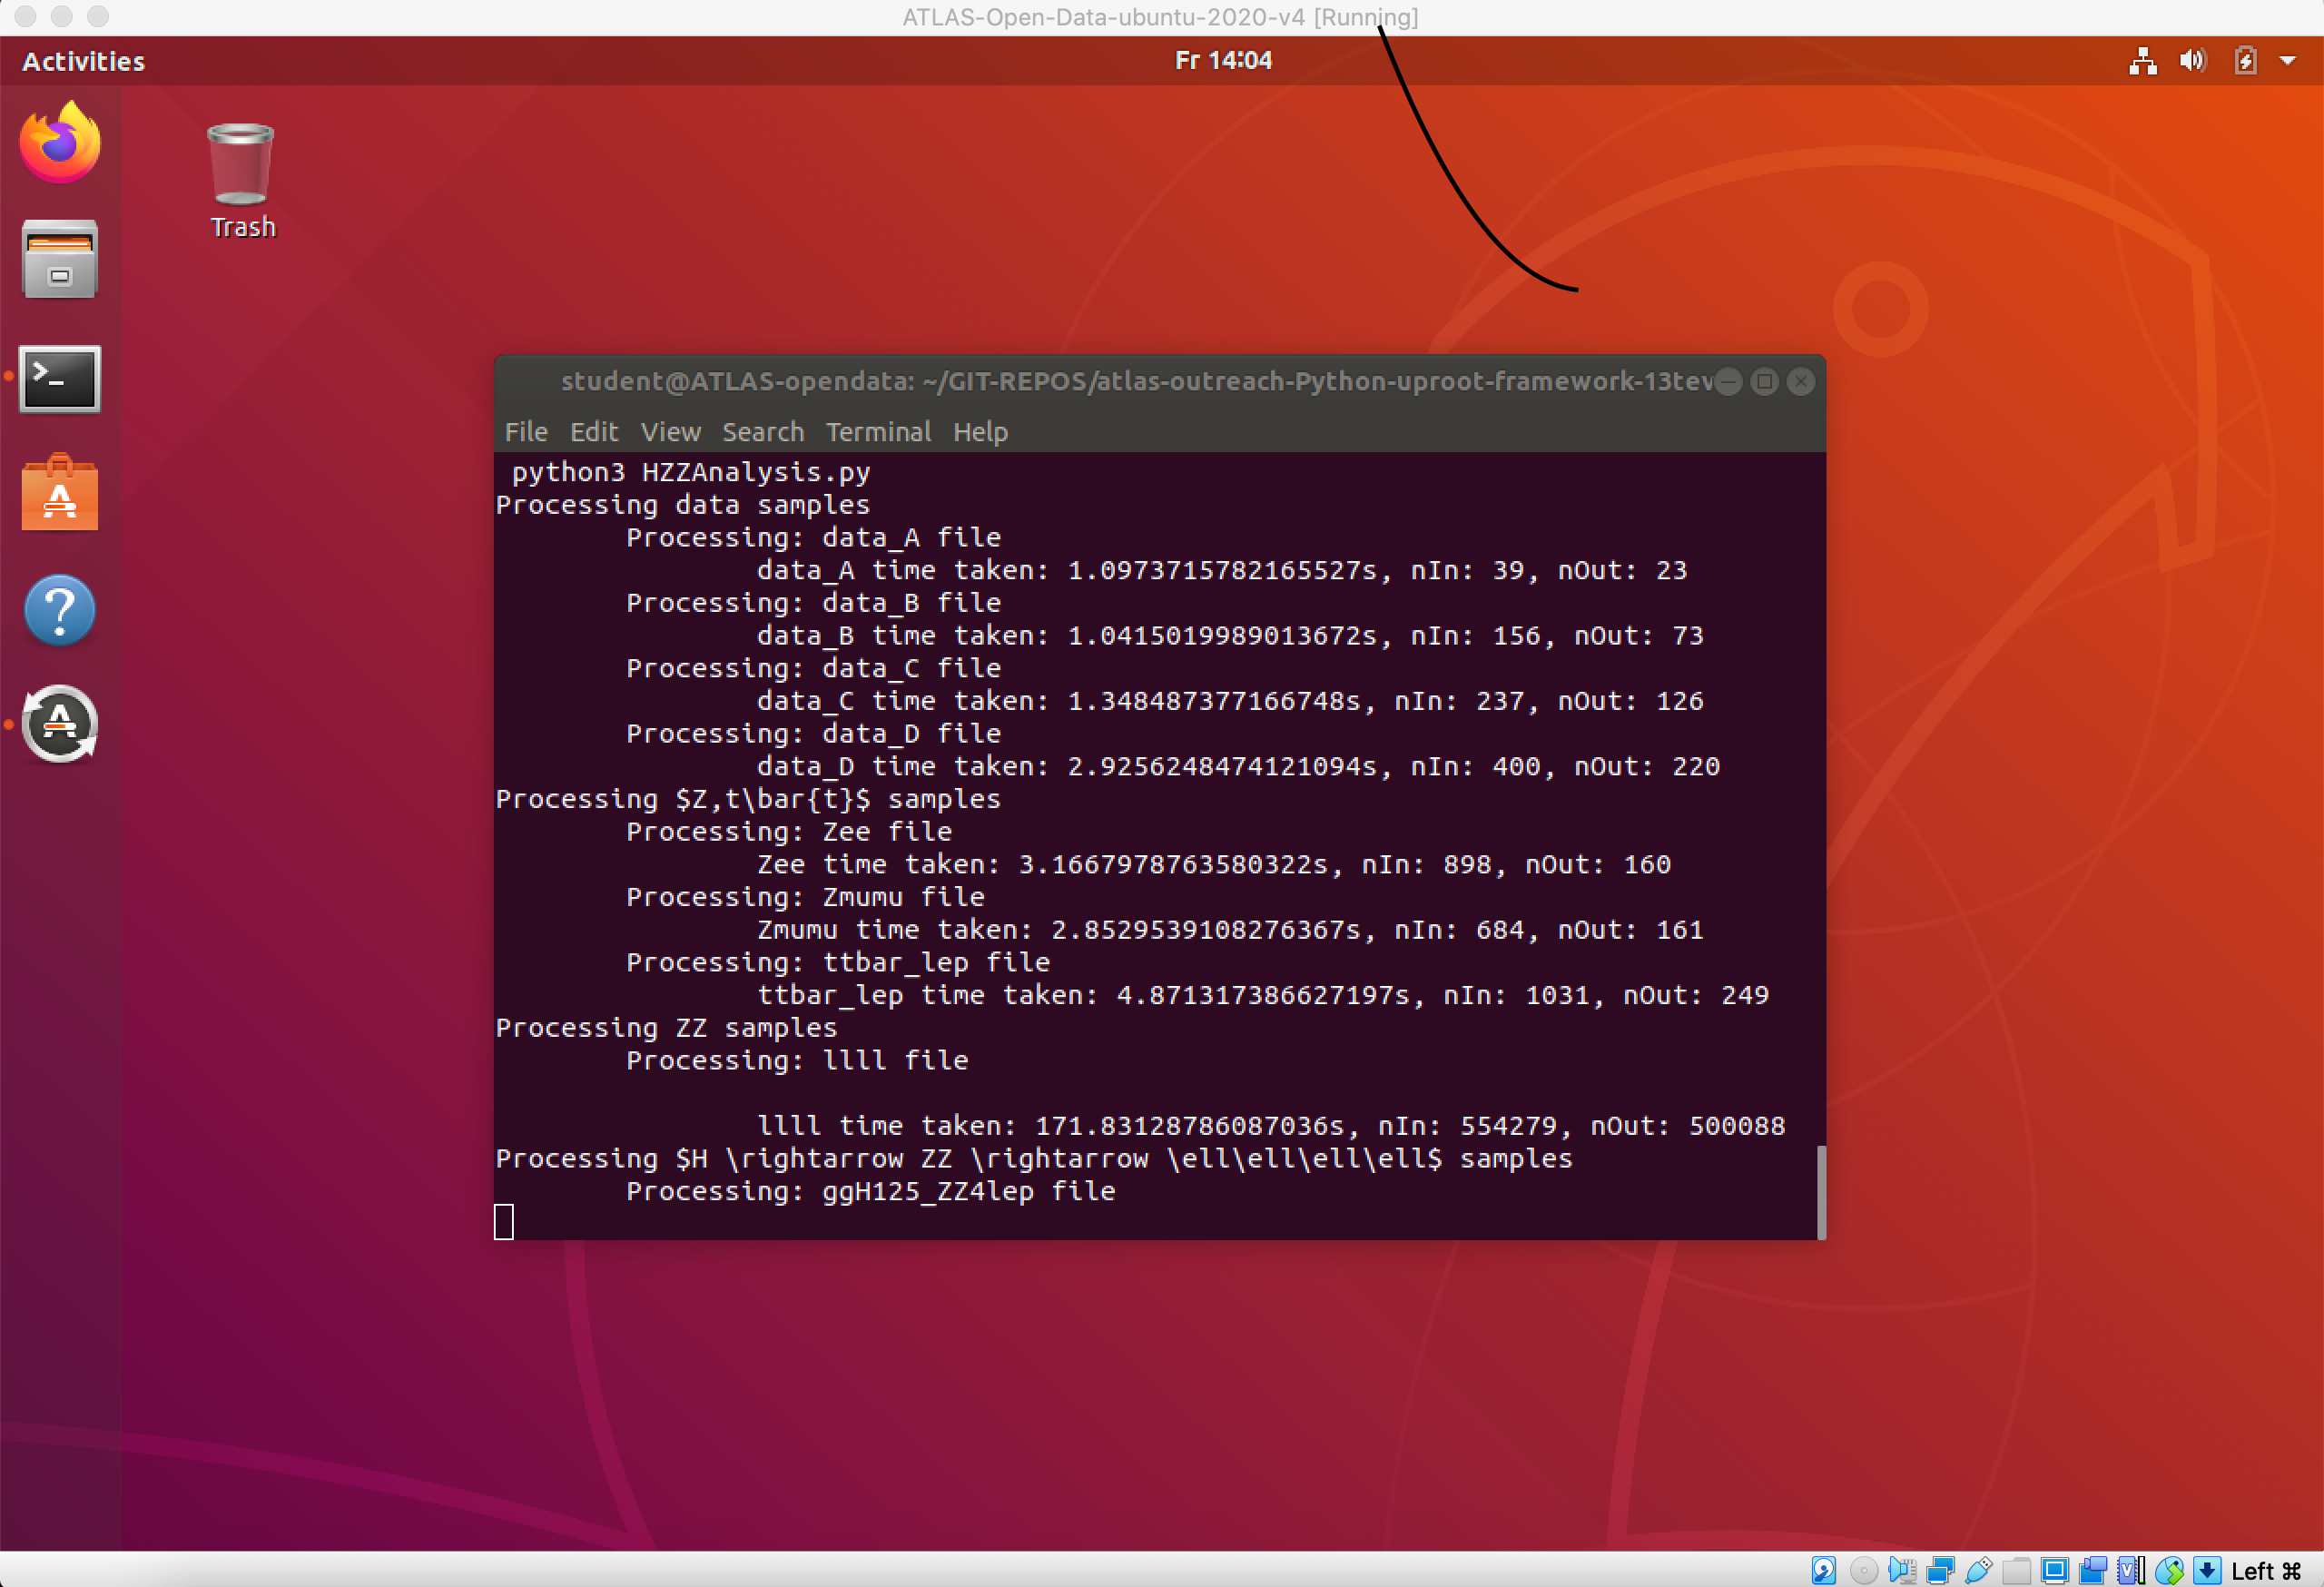
\includegraphics[width=0.7\columnwidth]{Figures/Running_HZZ.png}
	\label{fig:running_HZZ}
	\caption{Running HZZAnalysis.py from the ATLAS Virtual Machine terminal.}
\end{figure}

At the end of the running, you should have a file called \verb|HZZ_mlll.pdf|. You can see it by typing \verb|evince  HZZ_mlll.pdf| in the virtual machine terminal. It will be very similar to what the notebook above has produced. 

You can edit this file, or (better) make a copy and then edit. The full list of variables available in the open data files is available at \href{http://opendata.atlas.cern/release/2020/documentation/datasets/dataset13.html}{this link.}. For most of them, the variable description should help to understand what they are. Some others will not be used in this experiment. Finally, the meaning of some variables will become clear later. 

You are now ready to start with your experiments!


\subsection{ATLAS Virtual Machine}

 In case you have problems getting this working on your laptop, you can try the ATLAS virtual machine, with instructions below. Full instructions on how to install the ATLAS virtual machine can be found on the \href{http://atlas.cern/resources/opendata}{ATLAS open data} web site\footnote{If you end up with an error ``VT -x Is disabled in teh BIOS for all CPU modes'',  you will need to enable virtualisation. You can find out how to do that by googleing ``[your machine] enable virtualisation'' (unfortunately instructions are laptop-specific).}. Full instructions on how to install the ATLAS virtual machine can be found on the \href{http://atlas.cern/resources/opendata}{ATLAS open data} web site. 

\begin{remark}
\textbf{ATLAS Virtual Machine:} Please follow the video about the \verb|VirtualBox| installation (if you do not have it already), then follow the instruction specific to the installation of the 13 TeV ATLAS Open Data virtual machine installation. 
\end{remark}

As the videos describe, after having started the ATLAS virtual machine, you will be able to type \verb|localhost:8888| in your browser. 

That will show you the directories and files which are there in the virtual machine. If you now go back to the ATLAS virtual machine window, and there you open a terminal, and type \verb|ls|, you will see the same view. Please go to 

\verb|GIT-REPOS/GIT-REPOS/atlas-outreach-Python-uproot-framework-13tev|

If the directory is not there, you will need to clone the git repository from \href{https://github.com/atlas-outreach-data-tools/atlas-outreach-Python-uproot-framework-13tev}{this link} as described above. 



